
\section{Análisis teórico del circuito}
	En la Figura \ref{darlington_tp} se muestra el circuito implementado. 

\begin{figure}[H]
	\centering
		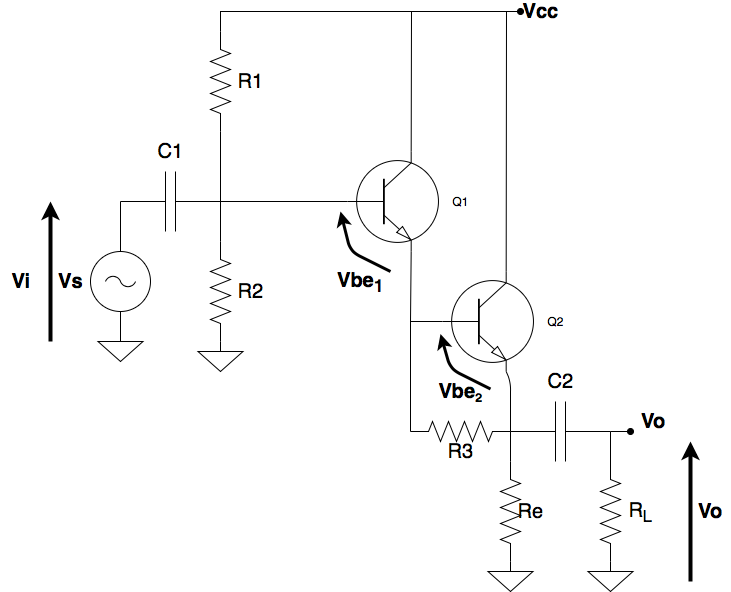
\includegraphics[scale=0.4]{./Imagenes/darlington_tp.png} \\
	\caption{Circuito de estudio en este trabajo, implementando un par Darlington.}
	\label{darlington_tp}
\end{figure}

La resistencia $R_3$ est\'a para que la corriente de emisor del primer transistor no vaya por completo a la base del segundo transistor, para evitar obtener $h_{fe}$ muy distintos para cada transistor, como se explica a continuaci\'on. La corriente del emisor del primer transistor es pr\'acticamente igual a la de su colector, por lo que es $h_{fe1}$ veces mayor a su corriente de base. Si no se coloca $R_3$, la corriente de base del segundo transistor es igual a la corriente de emisor del primero, por lo que al ser $I_{b2} >> I_{b1}$, se obtiene $I_{C2}>>I_{C1}$. Observando el gr\'afico \ref{icbeta} obtenido de la hoja de datos del transistor usado, se puede ver que el $h_{fe}$ cambia considerablemente al variar $I_C$. Por lo tanto, tendr\'iamos dos transistores con $h_{fe}$ distintos. Por otro lado, si $I_{C2} >> I_{C1}$, se podr\'ia llegar a obtener un valor de $I_{C2}$ mayor a 300mA, d\'onde el $h_{fe}$ disminuye por lo que se ve en el gr\'afico) y por lo tanto la ganancia tambi\'en. Por lo tanto, $R_3$ permite que parte de la corriente del emisor del primer transistor vaya por ah\'i hacia el emisor del segundo transistor, disminuyendo la corriente de base del segundo transistor, reduciendo los problemas mencionados.

\begin{figure}[H]
	\centering
	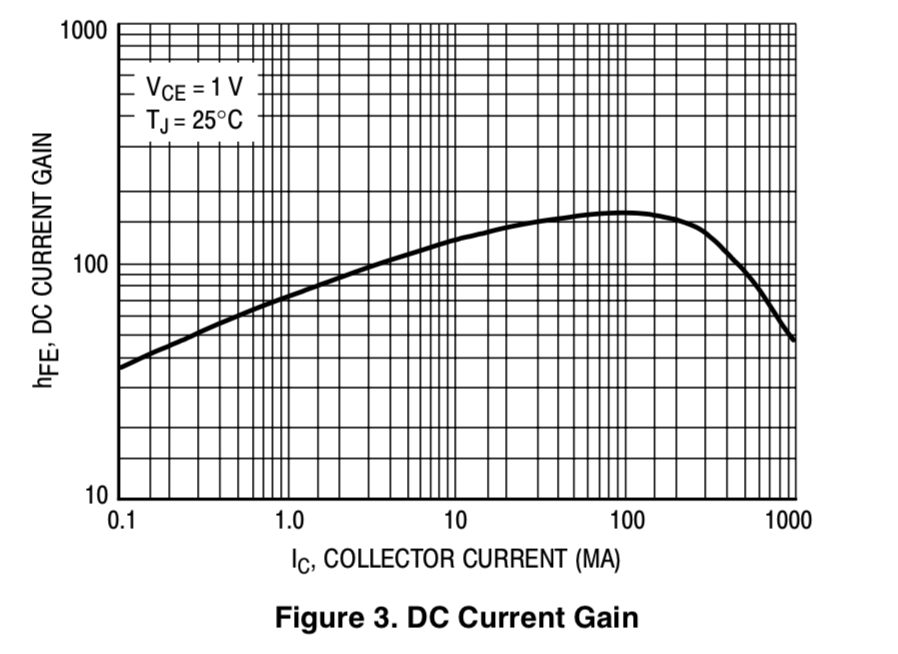
\includegraphics[scale=0.6]{./Imagenes/hfe.png} \\
	\caption{Gr\'afico de $h_{fe}$ en funci\'on de $I_C$, del transistor BC337-40.}
	\label{icbeta}
\end{figure}



	\subsection{Polarizaci\'on}
		En la Figura \ref{polarizacion} se muestra el modelo del circuito considerando que los capacitores representan circuitos abiertos, ya que en este caso se trabaja con tensión $V_{cc}$ continua. El mismo se esquematiza con el equivalente de Th\'evenin entre el nodo de base y masa.\\
		\begin{figure}[H]
			\centering
			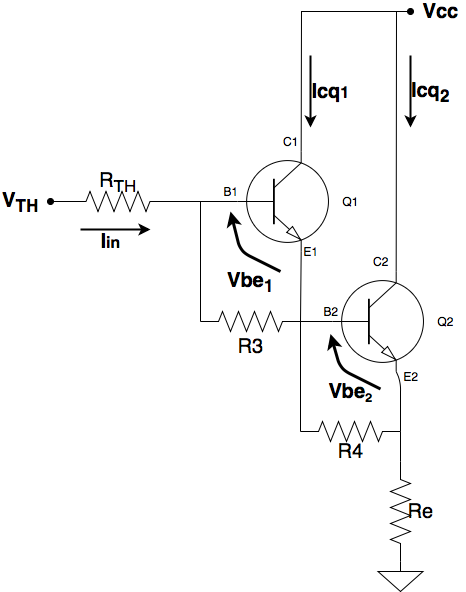
\includegraphics[scale=0.4]{./Imagenes/polarizacion.png} \\
			\caption{Circuito equivalente para el an\'alisis de polarizaci\'on.}
			\label{polarizacion}
		\end{figure}

Los valores utilizados para los cálculos son los de los componentes que usamos en la implementación del circuito, los cuales fueron elegidos en base a las simulaciones realizadas, con el fin de lograr un resultado óptimo. De esta forma, los valores de dichos componentes se listan en la Tabla \ref{tabla_valores}. Los transistores utilizados son BC337-40.

\begin{table}[H]
\centering
\begin{tabular}{ll}
\hline
\multicolumn{2}{l}{\begin{tabular}[c]{@{}l@{}}Parámetros\\   del circuito\end{tabular}} \\ \hline
$V_{cc}$                                     & $15V$                         \\
$R_1$                                         & $100 k\Omega$                           \\
$R_2$                                         & $330k\Omega$                              \\
$R_s$                                         & $10k\Omega$                             \\
$R_3$                                         & $10k\Omega$                          \\
$R_E$                                         & $4,7k\Omega$                               \\
$R_L$                                         & $1k\Omega$                           
\end{tabular}
\caption{Valores de los componentes utilizados}
\label{tabla_valores}  
\end{table}

El equivalente de Th\'evenin entre la base del primer transistor y masa se obtiene mediante:\\

	\begin{equation}
		\begin{cases}
		&V_{TH} = \frac{R_2}{R_1 + R_2} V_{CC} \approx  11,5V\\ \\
		&R_{TH} = R_1 // R_2 \approx 76,7k\Omega
		\end{cases}
		\label{Thevenin}
	\end{equation}

Recorriendo la malla de entrada se tiene que:
\begin{equation}
		V_{th}-I_{B1}R_{th}-V_{BEon_{1}}-V_{BEon_{2}}-R_{e}(I_{E_{2}}+I_{R_{3}})=0 
\end{equation}
Del nodo que conecta el emisor del primer transistor con la base del segundo, se relacionan las corrientes de los transistores:
\begin{equation}
		I_{B_{2}} = I_{E_{1}} - \frac{V_{BEon_{2}}}{R_{3}}
\end{equation}
Por último, de las ecuaciones de cada transistor, despreciando el efecto de las $I_{CB0}$ dado que se trabaja a temperatura ambiente, se verifica:

	\begin{equation}
		\begin{cases}
		Q_{1}: \, \, I_{E_{1}} = I_{B_{1}}(\beta_{1}+1)\\ \\
		Q_{2}: \, \, I_{E_{2}}=I_{B_{2}}(\beta_{2}+1)
		\end{cases}
	\end{equation}

Resolviendo dichas ecuaciones se llega a las siguientes expresiones para las corrientes de colector de ambos transistores:

	\begin{equation}
		\begin{cases}
		I_{cq_{1}}=\frac{V_{th}-V_{BEon_{1}}-V_{BEon_{2}}\left(1-\frac{R_{e}\beta_{2}}{R_{3}}\right)}{\frac{R_{th}}{\beta_{1}}+R_{e}\beta_{2}} = 93,54\mu A\\ \\
		I_{cq_{2}}=V_{th}\frac{1}{\frac{R_{th}}{\beta_{1}\beta_{2}}+R_{e}\frac{\beta_{2}+1}{\beta_{2}}}-V_{BEon_{1}}\frac{1}{\frac{R_{th}}{\beta_{2}}+R_{e}\beta_{1}}-V_{BEon_{2}}\left(\frac{\beta_{2}}{R_{3}}+\frac{\left(1-\frac{R_{e}\beta_{2}}{R_{3}}\right)\cdot(\beta_{1}+1)}{\frac{R_{th}}{\beta_{2}}+R_{e}\beta_{1}} \right) = 2,12mA
		\end{cases}
	\end{equation}

Por último, se puede verificar que ambos transistores queden correctamente polarizados mediante:

	\begin{equation}
		\begin{cases}
		V_{CEQ_{1}}=V_{CC}-V_{BEon_{2}}\left(1+\frac{R_{e}}{R_{3}}\right)-R_{e}I_{CQ_{2}} = 4,01V\\ \\
		V_{CEQ_{2}}=V_{CC}-V_{BEon_{2}}\frac{R_{e}}{R_{3}}-R_{e}I_{CQ_{2}} = 4,71V
		\end{cases}
	\end{equation}
	

Para los cálculos se utiliza $V_{BEon}=0.7(V)$ para ambos transistores. Con respecto a los $H_{FE}$, éstos dependen de las $I_{CQ}$ según la \href{https://pdf1.alldatasheet.com/datasheet-pdf/view/171970/ONSEMI/BC337-40.html}{hoja de datos del fabricante}, con lo que son distintos para cada transistor. Tomando inicialmente el $h_{fe}$ mínimo de la hoja de datos, e iterando para los valores de $I_{CQ}$ obtenidos, se llega a que:
	\begin{equation*}
		\begin{cases}
		 h_{fe1} = 47\\
		 h_{fe2} = 90
		\end{cases}
	\end{equation*}
Reemplazando además por los valores de los componentes utilizados, se hallan los valores de $I_{CQ1}$, $I_{CQ2}$, $V_{CEQ1}$ y $V_{CEQ2}$, detallados en la Tabla \ref{tabla_valores_polarizacion}.

\begin{table}[H]
	\centering
\begin{tabular}{ll}
\multicolumn{2}{l}{Polarización} \\ \hline
$I_{CQ1}$          & $93,54\mu A$       \\
$I_{CQ2}$        & $2,12mA$        \\
$V_{CEQ1}$         & $4,01V$       \\
$V_{CEQ2}$         & $4,71V$      
\end{tabular}
\caption{Valores hallados para las componentes de polarizacion.}
\label{tabla_valores_polarizacion}  
\end{table}


	\subsection{Modelo incremental}
	
	Los estimadores para los parámetros del modelo incremental de cada transistor se detallan a continuación.

		\begin{equation}
			\begin{cases}
			\widehat{r_{e}}=\frac{V_{T}}{I_{CQ}}\\
			{\widehat{h}_{ie}}=(\beta+1)R_{e}\\	
			{\widehat{g}_m}=\frac{1}{r_{e}}\\
			{\widehat{h}_{fe}}= \beta_{DC}\\
			\widehat{\frac{1}{h_{oe}}}= \infty
			\end{cases}
			\label{mod_inc_ecs}
		\end{equation}
		
	Se utiliza la ganancia de continua como estimador dado que las hojas de datos no especifican un valor para $h_{fe}$. Utilizando los valores de las corrientes de polarización y $h_{fe}$ de cada transistor, se obtienen los siguientes valores:
	

	\begin{table}[h!]
		\centering
		\begin{tabular}{c c c}%
			\bfseries Estimadores & Q1 & Q2 \\ \hline
			$\widehat{g}_m$ & $3,60 \frac{mA}{V}$  & $80\frac{mA}{V}$ \\
			$\widehat{h}_{ie}$ & $13,34k\Omega$ &$1,12k\Omega$ \\
			$\widehat{r}_{e}$& $277,96\Omega$ &$12,26\Omega$ \\
			\hline
		\end{tabular}
		\caption{Estimadores correspondientes al modelo incremental, para los transistores Q1 y Q2.}
		\label{avolf}
	\end{table}
	
	\subsection{Circuito incremental}
	
	En la Figura \ref{circ_incremental} se muestra el circuito incremental. Las resistencias de salida $1/h_{oe}$ de cada transistor se desprecian en los cálculos ya que hacerlo no introduce un error considerable y simplifica las operaciones.
		\begin{figure}[H]
			\centering
			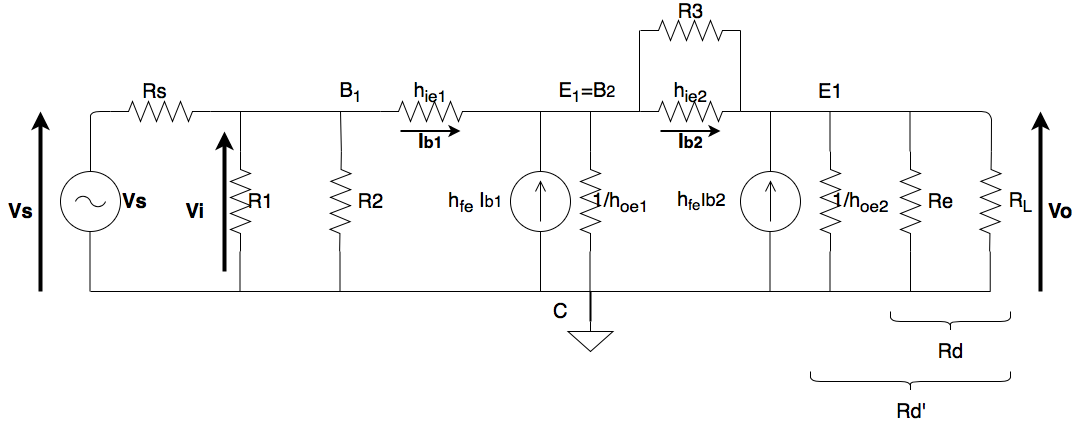
\includegraphics[scale=0.4]{./Imagenes/circ_incremental.png} \\
			\caption{Circuito equivalente para el an\'alisis del circuito incremental.}
			\label{circ_incremental}
		\end{figure}

En la Tabla \ref{tabla_valores_incremental} se muestran los valores utilizados en esta sección para luego calcular las ganancias e impedancias del circuito.

\begin{table}[H]
\centering
\begin{tabular}{ll}
\multicolumn{2}{l}{Modelo incremental} \\ \hline
$V_T$              & 26mV             \\
$h_{fe1}$           & 47            \\
$h_{fe2}$           & 90            \\
$h_{ie1}$            & 13,34$k\Omega$            \\
$h_{ie2}$           & 1,12$k\Omega$             \\
\end{tabular}
\label{tabla_valores_incremental} 
\end{table}

Para poder resolver el circuito fácilmente, se agrupa en paralelo la resistencia $R_3$ con $hie2$. Para poder hacerlo, se debe también adaptar la fuente de corriente del segundo transistor por la que circula por el paralelo de las resistencias de la siguiente forma. Además, se agrupan en paralelo $R_e$ y $R_L$. Para éstas consideraciones se calculan los siguientes parámetros:

	\begin{equation}
		\begin{cases}
		h_{fe2}^{*}=h_{fe2}\frac{R_{3}}{R_{3}+h_{ie2}} \\
		h_{ie2}^{*}=h_{ie2}//R_{3} \\
		R_{d}=R_{e}//R_{2}
		\end{cases}
		\label{mod_inc_ecs}
	\end{equation}

Reemplazando por los valores correspondientes se obtienen los siguientes valores:

\begin{table}[H]
\centering
\begin{tabular}{ll}
\multicolumn{2}{l}{Simplificaciones} \\ \hline
$h_{fe2}^*$          & 80,96           \\
$h_{ie2}^*$   & $1k\Omega$\\
$R_d$    & $824,56\Omega$  
\end{tabular}      
\end{table}

A partir del circuito y de los cálculos anteriores, se puede ver que las expresiones para las impedancias que se ven a la entrada del primer transistor, del amplificador y del sistema se ven representadas por las ecuaciones que se muestran a continuación, utilizando pasaje a nivel de corriente. 

	\begin{equation}
		\begin{cases}	
		R_{i}=hie_{1}+(hfe_{1}+1)hie_{2}^{*}+(hfe_{2}^{*}+1)(hfe_{1}+1)R_{d} \\
		R_{ia}=R_{i} // R_{th} \\
		R_{is}=R_{s}+R_{ia}
		\end{cases}
		\label{mod_inc_ecs}
	\end{equation}

De donde reemplanzando por los valores ya calculados se obtienen las impedancias de entrada:

\begin{table}[H]
\centering
\begin{tabular}{ll}
\multicolumn{2}{l}{\begin{tabular}[c]{@{}l@{}}Impedancias\\   de entrada\end{tabular}} \\ \hline
$R_i$                                      & 3,31$M\Omega$                                     \\
$R_{ia}$                                     & 75$k\Omega$                                    \\
$R_{is}$                                    & 85$k\Omega$                                   
\end{tabular}
\end{table}

Para el cálculo de la ganancia de tensión del sistema primero se calcula:

	\begin{equation}
		\begin{cases}	
		\frac{V_{o}}{ib_{2}^{*}}=R_{d}(hfe_{2}^{*}+1) \\
		\frac{V_{i}}{V_{s}}=\frac{R_{ia}}{R_{ia}+R_{s}}
		\end{cases}
		\label{mod_inc_ecs}
	\end{equation}

Así la ecuación de la ganancia en tensión del sistema se puede expresar de la siguiente forma. \\

	\begin{equation}	
		\Delta _{vs}=\frac{V_{o}}{V_{s}}=\frac{V_{o}}{ib_{2}^{*}}\cdot\frac{ib_{2}^{*}}{ib_{1}}\cdot\frac{ib_{1}}{V_{i}}\cdot\frac{V_{i}}{V_{s}}=R_{d}(hfe_{2}^{*}+1)(hfe_{1}+1)\frac{1}{R_{i}}\frac{Ria}{Ria+Rs}
		\label{mod_inc_avs}
	\end{equation}

Finalmente, se llega a los valores de las ganancias de tensión del amplificador y del sistema:

\begin{table}[H]
\centering
\begin{tabular}{ll}	
\multicolumn{2}{l}{\begin{tabular}[c]{@{}l@{}}Ganancias\\   de tension\end{tabular}} \\ \hline
$\Delta_{V}$                                       & 0,981                                     \\
$\Delta_{VS}$                                      & 0,866                                    
\end{tabular}
\end{table}

Al ser la configuración colector común se esperaba una ganancia de tensión menor a 1. De éste resultado se puede observar una ventaja de la configuración Darlington con respecto al colector común con un solo transistor, ya que éste último no puede llegar valores de ganancia de tensión superiores al 80\%.\\
Para el cálculo de la ganancia de corriente se utiliza:

	\begin{align*}
		\Delta _{i} &= \frac{I_{Rd}}{ib_{1}}=(hfe_{2}^{*}+1)(hfe_{1}+1) \\
%
	\Delta_{is} &= \frac{I_{Rd}}{I_{Rs}}\cdot\frac{I_{b_{1}}}{I_{Rs}}=\frac{R_{th}}{R_{th}+R_{i}}\Delta_{i} \\
%
		\Delta_{is}^{\, \, \,'} &= \frac{I_{Rl}}{I_{Rs}}=\frac{I_{Rl}}{I_{Rd}}\cdot\frac{I_{Rd}}{I_{Rs}}=\frac{R_{e}}{R_{e}	+R_{2}}\Delta_{is}
%
		\label{mod_inc_ais}
	\end{align*}


Donde $\Delta_{i}$ es la ganancia de corriente, $\Delta_{is}$ es la ganancia de corriente del sistema y $\Delta_{is}^{\, \, \,'}$ es la ganancia de corriente del sistema sobre la carga. En $\Delta_{i}$ se puede apreciar la gran ganancia de corriente que tiene esta configuración, ya que se multiplican las ganancias de cada transistor. Los valores de las mismas se muestran en la siguiente tabla:

\begin{table}[H]
\centering
\begin{tabular}{ll}
\multicolumn{2}{l}{\begin{tabular}[c]{@{}l@{}}Ganancias\\   de corriente\end{tabular}} \\ \hline
$\Delta_I$                                       & 3934,08                                     \\
$\Delta_{IS}$                                      & 89,27                                       \\
$\Delta_{is}'$                                     & 73,61                                      
\end{tabular}
\end{table}

Para la resistencia de salida, se pasiva la entrada, se coloca a la salida una fuente $V_{op}$ con el terminal positivo a masa, y se calcula la corriente $I_{op}$ que circula por dicha fuente. Las siguientes relaciones se utilizan para el cálculo:

	\begin{equation}
		\begin{cases}	
		V_{op}=I_{B1}( R_{s}//R_{th}+h_{ie1} + hfe_{1}+1)hie_{2}^{*}) \\
		I_{op}=I_{B1}(hfe_{1}+1)(hfe_{2}^{*}+1)\\
		r_{o}=\frac{V_{op}}{I_{op}}=\frac{R_{s}//R_{th}+hie1+(hfe1+1)hie_{2}^{*}}{(hfe_{1}+1)(hfe_{2}^{*}+1)}\\
		r_{oa}=R_{e}//r_{o}\\
		r_{os}=r_{oa}//R_{L}
		\end{cases}
		\label{mod_inc_ro}
	\end{equation}

Reemplazando por los valores de las variables involucradas en la ecuación, se obtienen los valores de las resistencias de salida vistas a la salida del segundo transistor, a la salida del amplificador y luego de la carga.

\begin{table}[H]
\centering
\begin{tabular}{ll}
\multicolumn{2}{l}{Impedancias de salida} \\ \hline
$r_o$                &   $17,9\Omega$        \\
$r_{oa}$              &  $17,83\Omega$      \\
$r_{os}$               &  $17,52\Omega$              
\end{tabular}
\end{table}
